\section{Unique Game Conjecture}

\subsection{Unique Label Cover}

    It is an optimization problem.

    We are given a \textit{bipartite graph} $G((V,W), E)$ (see~\nameref{subsubsec:bipartitegraph}), and given a set of labels $[m] = \{1, 2, \dots, m\}$, and $\forall e = \{ v,w \} \in E$ a permutation $\pi_{vw} : [m] \rightarrow [m]$.

    Find an assignment of labels to the vertices, $\phi : V \cup W \rightarrow [m]$, s.t.~the set $S$ of satisfied edges is as large as possible.
    \[ S = \{ v,w \} \in E \st v \in V \wedge w \in W \wedge \pi_{vw}(\phi(v)) = \phi(w) \]

\subsection{Unique Games Conjecture}
    Formulated by Khot in 2002.

    For each $\varepsilon > 0$, it is NP-Hard to determine if, in a Unique Label Cover problem, with $m = m(\varepsilon)$ labels, if:
    \begin{itemize}
        \item Each assignment of labels (each solution) satisfies no more than $\varepsilon \cardinality{E}$ edges, or
        \item There exists an assignment (a solution) which satisfies at least $(1-\varepsilon) \cardinality{E}$ edges
    \end{itemize}

    From this conjecture, came a bunch of theorems stating that, if the UGC holds, than some problem is NP-Hard to approximate better than a specific value. Let us see a couple of examples.

    \begin{theorem}
        If the UGC holds, then $\forall \varepsilon > 0$, it is NP-Hard to approximate Max-Cut to $\alpha_{GW} - \varepsilon$.
    \end{theorem}

    \begin{theorem}
        If the UGC holds, then $\forall \varepsilon > 0$, is it NP-Hard to approximate Vertex-Cover to $2 - \varepsilon$.
    \end{theorem}


\subsection{Constraint Satisfaction Problems (CSPs)}
    CSPs of a constant arity, on a constant-sized alphabet, can be optimally approximated via a SDP-based algorithm in polytime, if the UGC holds.


\subsection{Sparsest Cut problem}
    Sparsest Cut is not a CSP.\@

    Given an undirected graph $G(V,E)$, find a subset $\emptyset \subset S \subset V$ that minimizes
    \[ \Psi(S) = \dfrac{\cardinality{Cut(S, V \setminus S)}}{\cardinality{S} \cdot \cardinality{V \setminus S}} \]

    Let us consider the Sparsest Cut problem for \textbf{Erd\H{o}s-Renyi random graphs}.
    To sample an E-R r.g., one can use the algorithm \ref{alg:er_rg}.

    \begin{algorithm}
    \caption{E-R random graph $G(n,p)$}\label{alg:er_rg}
    \begin{algorithmic}%[1]
        \State$S \gets [n]$\@
        \State$E \gets \emptyset$\@
        \For{each $\{i,j\} \in \binom{V}{2}$ }
            \State flip an iid coin with head probability $p$\@
            \If{coin is heads}
                \State $E \gets E \cup \{i,j\}$
            \EndIf\@
        \EndFor\@

        \State\Return~$G(V,E)$
    \end{algorithmic}
\end{algorithm}

    %$\expected[\cardinality{Cut(S, V \setminus S)}] =
    %\sum_{i \in S} \sum_{j \in V \setminus S} \prob[\{ i,j \} \in E] =
    %\sum_{i \in S} \sum_{j \in V \setminus S} p =
    %\cardinality{S} \cdot \cardinality{V \setminus S} \cdot p$

    \begin{equation*}
        \begin{split}
            \expected[\cardinality{Cut(S, V \setminus S)}] &=\\
                &= \sum_{i \in S} \sum_{j \in V \setminus S} \prob[\{ i,j \} \in E] =\\
                &= \sum_{i \in S} \sum_{j \in V \setminus S} p = \cardinality{S} \cdot \cardinality{V \setminus S} \cdot p
        \end{split}
    \end{equation*}

    Thus, $\expected_{G \thicksim G(n,p)}[\Psi(S)] =
    \dfrac{\expected[\cardinality{Cut(S, V \setminus S)}]}{\cardinality{S} \cdot \cardinality{V \setminus S}} =
    \dfrac{ \cardinality{S} \cdot \cardinality{V \setminus S} \cdot p}{\cardinality{S} \cdot \cardinality{V \setminus S}} = 
    p$

    We have concluded that
    \[ 0 \leq \cardinality{Cut(S, V \setminus S)} \leq \cardinality{S} \cdot \cardinality{V \setminus S} \]

    This implies that
    \[ \Psi(S) \in [0,1] \]

    Observe that, if $\Psi(S) = 0 \rightarrow$ $S$ is disconnected from $V \setminus S$.

    Our \textit{objective function} is
    \[ \Psi^* = \min_{\emptyset \subset S \subset V} \Psi(S) \]

    \textbf{Leighton-Rao} algorithm for Sparsest-Cut:
    \begin{itemize}
        \item Based on an LP
        \item Geometry plays a pivotal role in its analysis
        \item The algorithm is, essentially, a series of geometric reductions
    \end{itemize}


\subsection{Metrics}

    \begin{definition}[Metric]
        A metric $d$ on a set $S$ is a function $d : S \times S \rightarrow \mathbb{R}$, s.t.:
        \begin{enumerate}
            \item $d(X,Y) = d(Y,X)$, $\forall X,Y \in S$
            \item $d(X,X) = 0$, $\forall X \in S$
            \item $d(X,Y) + d(Y,Z) \geq d(X,Z)$, $\forall X,Y,Z \in S$ (Triangle inequality)
        \end{enumerate}
    \end{definition}

    \begin{definition}[Elemetary-cut metric]
        The elementary-cut metric $d_T : S \times S \rightarrow \mathbb{R}$, for $T \subseteq S$, is defined as
        \begin{equation}
            d_T(X,Y) = 
            \begin{cases}
                1 & \text{if } \cardinality{\{X,Y\} \in T } = 1\\
                0 & \text{o/w}
            \end{cases}
        \end{equation}
    \end{definition}

    \begin{lemma}
        If $d_T : S \times S \rightarrow \mathbb{R}$ is an elementary-cut metric, then $d_T$ is a metric.
    \end{lemma}

    \begin{proof}
        Axioms $1.$ and $2.$ are trivial to verify.

        Let $X,Y,Z \in S$:
        \begin{itemize}
            \item if $X,Y,Z \in T$, then $0 = d_T(X,Y) + d_T(Y,Z) \geq d_T(X,Z) = 0$
            \item if $X,Y,Z \not\in T$, then $0 = d_T(X,Y) + d_T(Y,Z) \geq d_T(X,Z) = 0$
        \end{itemize}

        It remains a third case, itself subdivided in three other subcases.

        Assume $\exists A \in \{ T, S \setminus T \}$ s.t.~exactly one of $X,Y,Z$ is in $A$; i.e.~we divide $X,Y$ and $Z$ in the two partitions of $S$.
        \begin{itemize}
            \item if $X \in A$, then $1 = d_T(X,Y) + d_T(Y,Z) \geq d_T(X,Z) = 1$
            \item if $Z \in A$, then $1 = d_T(X,Y) + d_T(Y,Z) \geq d_T(X,Z) = 1$
            \item if $Y \in A$, then $2 = d_T(X,Y) + d_T(Y,Z) \geq d_T(X,Z) = 0$
        \end{itemize}
    \end{proof}

    We want to argue that the Sparsest Cut problem is an optimization problem, over elementary-cut metrics.
    That is, the goal is to minimize $\phi(d_T)$, where $d_T : V \times V \rightarrow \mathbb{R}$ is an elementary-cut metric over $V$, and
    \[ \phi(d_T) = \dfrac{\sum_{\{x,y\} \in E} d_T(X,Y)}{\sum_{\{x,y\} \in \binom{V}{2}} d_T(X,Y)} \]

    \begin{lemma}\label{lemma:metric2}
        If $d_T$ is an elementary-cut metric over $V$, then
        \[ \phi(d_T) = \dfrac{\cardinality{Cut(S, V \setminus S)}}{\cardinality{T} \cdot \cardinality{V \setminus T}} \]
    \end{lemma}

    Let $P$ be any predicate. $[P]$ has value $1$ is $P$ is true, and $0$ if $P$ is false.

    \begin{proof}
        %$\phi(d_T) =
        %\dfrac{\sum_{\{x,y\} \in E} d_T(X,Y)}{\sum_{\{x,y\} \in \binom{V}{2}} d_T(X,Y)} = 
        %\dfrac{\sum_{\{x,y\} \in E} [X \in T \text{ xor } Y \in T]}{\sum_{\{x,y\} \in \binom{V}{2}} [X \in T \text{ xor } Y \in T]} = $

        %$\dfrac{\cardinality{Cut(T, V \setminus T)}}{\cardinality{T} \cdot \cardinality{V \setminus T}}$

        \begin{equation*}
            \begin{split}
                \phi(d_T)   &=\\
                            &= \dfrac{\sum_{\{x,y\} \in E} d_T(X,Y)}{\sum_{\{x,y\} \in \binom{V}{2}} d_T(X,Y)} = \dfrac{\sum_{\{x,y\} \in E} [X \in T \text{ xor } Y \in T]}{\sum_{\{x,y\} \in \binom{V}{2}} [X \in T \text{ xor } Y \in T]} =\\
                            &= \dfrac{\cardinality{Cut(T, V \setminus T)}}{\cardinality{T} \cdot \cardinality{V \setminus T}}
            \end{split}
        \end{equation*}
    \end{proof}

    \begin{definition}[Cut metric]
        Let $d_{T_1}, d_{T_2}, \dots, d_{T_k} : V \times V \rightarrow \mathbb{R}$ be elementary cut metric, and let $\lambda_1, \lambda_2, \dots, \lambda_k > 0$, then $d : V \times V \rightarrow \mathbb{R}$ defined as
        \[ d(X,Y) = \sum_{i=1}^{k}(\lambda_i \cdot d_{T_i}(X,Y)) \]
        is a cut metric.
    \end{definition}

    Cut metric are less "integral" (more "fractional"/flexible) than elementary cut metrics.

    \begin{lemma}\label{lemma:metric3}
        Let $d$ be a cut metric with cuts $T_1, T_2, \dots, T_k$, then
        \[ \phi(d) \geq \min_{i \in [k]} \phi(d_i) \]
    \end{lemma}

    Then, minimizing over cut metrics is equivalent to minimizing over elementary-cut metrics.

    \begin{proof}
        Since $d$ is a cut metric with cuts $T_1, \dots, T_k$, $\exists \lambda_1, \lambda_2, \dots, \lambda_k > 0$ s.t. $d(X,Y) = \sum_{i=1}^k(\lambda_i \cdot d_{T_i}(X,Y))$, $\forall X,Y \in V$.

        Then,
        %$\phi(d) =
        %\dfrac{\sum_{\{u,v\} \in E} d(u,v)}{\sum_{\{u,v\} \in \binom{V}{2}} d(u,v)} = 
        %\dfrac{\sum_{\{u,v\} \in E} \sum_{i=1}^{k} (\lambda_i \cdot d_{T_i}(u,v))}{\sum_{\{u,v\} \in \binom{V}{2}} \sum_{i=1}^{k} (\lambda_i \cdot d_{T_i}(u,v))} = 
        %\dfrac{\sum_{i=1}^{k} \sum_{\{u,v\} \in E} (\lambda_i \cdot d_{T_i}(u,v))}{\sum_{i=1}^{k} \sum_{\{u,v\} \in \binom{V}{2}} (\lambda_i \cdot d_{T_i}(u,v))}$

        \begin{equation*}
            \begin{split}
                \phi(d) &= \dfrac{\sum_{\{u,v\} \in E} d(u,v)}{\sum_{\{u,v\} \in \binom{V}{2}} d(u,v)} = \dfrac{\sum_{\{u,v\} \in E} \sum_{i=1}^{k} (\lambda_i \cdot d_{T_i}(u,v))}{\sum_{\{u,v\} \in \binom{V}{2}} \sum_{i=1}^{k} (\lambda_i \cdot d_{T_i}(u,v))} =\\
                        &= \dfrac{\sum_{i=1}^{k} \sum_{\{u,v\} \in E} (\lambda_i \cdot d_{T_i}(u,v))}{\sum_{i=1}^{k} \sum_{\{u,v\} \in \binom{V}{2}} (\lambda_i \cdot d_{T_i}(u,v))}
            \end{split}
        \end{equation*}

        We now claim that, if $a_i, b_i > 0$, $\forall i \in [k]$, then
        \[ \dfrac{\sum_{i=1}^k a_i}{\sum_{i=1}^k b_i} \geq \min_{i \in [k]} \dfrac{a_i}{b_i} \]

        Let $\rho = \min_{i \in [k]} \dfrac{a_i}{b_i}$.

        Then
        $\dfrac{\sum_{i=1}^k a_i}{\sum_{i=1}^k b_i} = 
        \dfrac{\sum_{i=1}^k b_i \frac{a_i}{b_i}}{\sum_{i=1}^k b_i} \geq
        \dfrac{\sum_{i=1}^k b_i \rho}{\sum_{i=1}^k b_i} =
        \rho$

        Thus the claim is proved.

        Now,
        \[ \phi(d) \geq \min_{i \in [k]} \dfrac{\sum_{\{u,v\} \in E} (\lambda_i \cdot d_{T_i}(u,v))}{\sum_{\{u,v\} \in \binom{V}{2}} (\lambda_i \cdot d_{T_i}(u,v))} = \min_{i \in [k]} \phi(d_{T_i}) \]
    \end{proof}

    \begin{corollary}
        \[ \min_{\substack{d\\ d \text{  a cut metric}}} \phi(d) = \min_{\substack{d_T\\ d_T \text{ an elem. cut metric}}} \phi(d_T) = \Psi^*  \]
    \end{corollary}

    \begin{proof}
        Follows from Lemma~\ref{lemma:metric2} and Lemma~\ref{lemma:metric3}.
    \end{proof}

    \begin{exercise}
        Prove that each cut metric $d$ is a metric.
    \end{exercise}

    \begin{definition}[Normed metric]
        Given $\underbar{X}, \underbar{Y} \in \mathbb{R}^d$,
        \[ \ell_p(\underbar{X}, \underbar{Y}) = \sqrt[p]{\sum_{t=1}^{d} \cardinality{X(t) - Y(t)}^p} \]
    \end{definition}

    \begin{theorem}
        $\ell_p$ is a metric over $\mathbb{R}^d$, $\forall d \geq 1$, $\forall p \geq 1$.
    \end{theorem}

    We define $\ell_\infty$ as
    \[ \ell_\infty(\underbar{X}, \underbar{Y}) = \max_{t \in [d]} \cardinality{X(t) - Y(t)} = \lim_{p \rightarrow \infty} \ell_p(\underbar{X}, \underbar{Y}) \]

    We are interested in some specific metrics.
    Consider $\ell_1$, called \textit{Manhattan distance}, which has some nice properties.
    It is, essentially, just a linear function with absolute values.
    \[ \ell_1(\underbar{X}, \underbar{Y}) = \cardinality{\underbar{X} - \underbar{Y}}_1 = \sum_{t=1}^{d} \cardinality{X(t) - Y(t)} \]

    \begin{lemma}\label{lemma:metric4}
        If $d : V \times V \rightarrow \mathbb{R}$ is a cut metric over $k$ cuts, then $f : V \rightarrow \mathbb{R}^k$ s.t. $d(X,Y) = \cardinality{f(X) - f(Y)}_1$, $\forall X,Y \in V$.

        If $X \subseteq \mathbb{R}^d$ is finite, then the $l-1$-metric over $X$ can be represented by a cut metric over $k = (\cardinality{X}-1)d$ cuts.
    \end{lemma}

    \begin{proof}
        If $d$ is a cut metric, $\exists \lambda_1, \dots, \lambda_k > 0$, and $\emptyset \subset T_1, \dots, T_k \subset V$ s.t. $\forall \{u,v\} \in \binom{V}{2}$
        \[ d(u,v) = \sum_{i=1}^{k}(\lambda_i d_{T_i}(u,v)) \]

        $\forall u \in V$, define $\underbar{X}_u \in \mathbb{R}^k$ ($\underbar{X}_u = f(u)$) as follows:
        \begin{equation}
            \underbar{X}_u(i) = 
            \begin{cases}
                \lambda_i   & \text{if } u \in T_i\\
                0           & \text{o/w}
            \end{cases}
        \end{equation}

        Let $u,v \in V$, then
        %$\cardinality{\underbar{X}_u - \underbar{X}_v}_1 =
        %\sum_{i=1}^{k}\cardinality{\underbar{X}_u(i) - \underbar{X}_v(i)} =
        %\sum_{i=1}^{k}([\cardinality{\{u,v\} \cap T} = 1] \cdot \lambda_i) =
        %\sum_{i=1}^{k}(d_{T_i}(u,v) \cdot \lambda_i) =
        %d(u,v)$

        \begin{equation*}
            \begin{split}
                \cardinality{\underbar{X}_u - \underbar{X}_v}_1 &= \sum_{i=1}^{k}\cardinality{\underbar{X}_u(i) - \underbar{X}_v(i)} = \sum_{i=1}^{k}([\cardinality{\{u,v\} \cap T} = 1] \cdot \lambda_i) =\\
                    &= \sum_{i=1}^{k}(d_{T_i}(u,v) \cdot \lambda_i) =\\
                    &= d(u,v)
            \end{split}
        \end{equation*}

        Now, suppose that we have $X \subseteq \mathbb{R}$.
        Let us start, for semplicity, with $d=1$.

        Suppose that the points that we want to embed in a cut metric are $(X_1), (X_2), \dots, (X_n)$.

        Let $\pi : [n] \rightarrow [n]$ be a permutation s.t. $X_{\pi(1)} \leq X_{\pi(2)} \leq \cdots \leq X_{\pi(n)}$.
        For each $j = 1, \dots, n-1$, let $S_j$ be defined as
        \[ S_j = \{ \pi(1), \pi(2), \dots, \pi(j) \} \]

        Moreover, $\lambda_j = X_{\pi(j+1)} - X_{\pi(j)}$.
        Then $\lambda_j \geq 0$, since $X_{\pi(j+1)} \geq X_{\pi(j)}$.

        For each $i < j$, it hold that
        %$\lambda_i  + \lambda_{i+1} + \cdots + \lambda_{j-1} = 
        %\sum_{t=1}^{n-1}(d_{S_t}(\pi(i), \pi(j)) \cdot \lambda_t) = 
        %(X_{\pi(j)} - X_{\pi(j-1)}) + (X_{\pi(j-1)} - X_{\pi(j-2)}) + \cdots + (X_{\pi(i+1)} - X_{\pi(i)}) = 
        %X_{\pi(j)} - X_{\pi(i)} = 
        %\cardinality{X_{\pi(j)} - X_{\pi(i)}}_1$

        \begin{equation*}
            \begin{split}
                \lambda_i  + \lambda_{i+1} + \cdots + \lambda_{j-1} &= \sum_{t=1}^{n-1}(d_{S_t}(\pi(i), \pi(j)) \cdot \lambda_t) =\\
                    &= (X_{\pi(j)} - X_{\pi(j-1)}) +\\
                    &+ (X_{\pi(j-1)} - X_{\pi(j-2)}) +\\
                    & \vdots\\
                    &+ (X_{\pi(i+1)} - X_{\pi(i)}) =\\
                    &= X_{\pi(j)} - X_{\pi(i)} = \cardinality{X_{\pi(j)} - X_{\pi(i)}}_1
            \end{split}
        \end{equation*}

        Thus, an $\ell_1$-metric $X$, over $d=1$ dimension, can be represented by a cut metric (over $\cardinality{X}-1$ cuts).
        In general, an $\ell_1$-metric over $d$ dimensions is equal to the sum of $d$ $\ell_1$-metrics over $1$ dimension each.

        Thus any $\ell_1$-metric $X$ over $d$ dimensions can be emebedded into a cut metric over $d(\cardinality{X}-1)$ cuts.
    \end{proof}

    \begin{corollary}
        \[ \min_{\substack{d\\ d \text{ a } \ell_1 \text{-metric}}} \phi(d) = \min_{\substack{d\\ d \text{  a cut metric}}} \phi(d) = \min_{\substack{d_T\\ d_T \text{ an elem. cut metric}}} \phi(d_T) = \min_{\emptyset \subset S \subset V} \Psi(S)  \]
    \end{corollary}

    Observe that
    \begin{equation}
        \begin{cases}
            \min \phi(d)\\
            d \text{ an } \ell_1 \text{-metric}
        \end{cases}
        \Longleftrightarrow
        \begin{cases}
            \min \sum_{\{u,v\} \in E} d(u,v)\\
            d \text{ an } \ell_1 \text{-metric}\\
            \sum_{\{u,v\} \in \binom{V}{2}} d(u,v) = 1
        \end{cases}
    \end{equation}

    \begin{theorem}[Bourgain, Linial et al.]
        Any metric on $n$ points can be embedded into $\ell_1$ (with $d = O(\log^2 n)$ dimensions) with "distortion" $O(\log n)$.
        Furthermore, the embedding can be obtained in polynomial time.
    \end{theorem}

    \begin{definition}[Distortion]
        If $d$ and $d'$ are metric over $V$, then if $\exists \alpha, \beta \geq 1$ s.t. $\forall x,y \in V$
        \[ \dfrac{d(x,y)}{\alpha} \leq d'(x,y) \leq \beta \cdot d(x,y) \]
        then the distortion of the pair $d,d'$ is not larget than $\alpha \cdot \beta$.
    \end{definition}


\subsection{Leighton-Rao algorithm}
    We now see an algorithm for approximating Sparsest, based on LP.

    Procedure:
    \begin{enumerate}
        \item Solve the metric LP
        \begin{equation}
            \begin{cases}
                \min \sum_{\{u,v\} \in E} X_{\{u,v\}}\\
                X_{\{u,v\}} + X_{\{v,w\}} \geq X_{\{u,w\}}          & \forall u,v,w \in V\\
                \sum_{\{u,v\} \in \binom{V}{2}} X_{\{u,v\}} = 1\\
                X_{\{u,v\}} \geq 0                                  & \forall \{u,v\} \in \binom{V}{2}
            \end{cases}
        \end{equation}
        \item Let $d$ be the resulting metric
        \item Apply Bourgain's theorem on $d$, to obtain a $\ell_1$-metric $d'$ that distorts $d$ by at most $O(\log n)$
        \item Apply the algorithm of Lemma~\ref{lemma:metric4} on $d'$, to obtain a cut metric $d''$ equal to $d'$ (i.e. no distortion)
        \item For each cut $T_i$ of $d''$, compute $\phi(d_{T_i})$
        \item Return $d''' = \argmin_{T_i} \phi(d_{T_i})$
    \end{enumerate}

    \begin{theorem}
        This algorithm return a $O(\log n)$ approximation to Sparset cut.
    \end{theorem}

    \begin{proof}
        $d$ minimizes the metric LP, then 
        \[ LP^* = \min_{\substack{\underbar{d}\\ \underbar{d} \text{ a cut-metric}}} \phi(\underbar{d}) = \min_{\substack{\underbar{d}\\ \underbar{d} \text{ a } \ell_1 \text{-metric}}} \phi(\underbar{d}) \]

        $d'$ distorts $d$ by at most $O(\log n)$: $\phi(d') \leq \phi(d) \cdot O(\log n) \leq OPT \cdot O(\log n)$.

        Moreover, $\phi(d'') = \phi(d') \leq OPT \cdot O(\log n)$.

        Finally, Lemma~\ref{lemma:metric3} guarantees that $\phi(d''') \leq \phi(d'') \leq OPT \cdot O(\log n)$.
    \end{proof}

    \begin{lemma}
        Each $\ell_1$-metric can be embedded into a cut metric with no distortion (i.e. distortion $1$).
        Each cut-metric can be embedded into $\ell_1$ with no distortion.
    \end{lemma}

    That is,
    \[ \ell_1 \sim \text{cut metrics} \]

    \begin{theorem}[Bourgain]
        Each metric on $n$ points can be embedded into $\ell_2$ with distortion $O(\log n)$.
    \end{theorem}

    This seems to indicate that $\ell_2$ is "weaker" than genearl metrics.
    Let us see an example of it.

    \begin{definition}
        For a connected undirected graph $G(V,E)$, the shortest path metric on $G$ is a metric over $V$ s.t.
        $\forall u,v \in V$, $d_G(u,v)$ is the number of edges of a shortest path from $u$ to $v$ in $G$.
    \end{definition}

    \begin{observation}
        The shortest path metric satisfies the triangle inequality.
    \end{observation}

    Consider the graph $C_4$, as in figure~\ref{fig:c4}.

    \begin{figure}[h]
        \centering
        %\begin{tikzpicture}
%
%    \def \n {5}
%    \def \radius {3cm}
%    \def \margin {8} % margin in angles, depends on the radius
%    
%    \foreach \s in {1,...,\n}
%    {
%      \node[draw, circle] at ({360/\n * (\s - 1)}:\radius) {$\s$};
%      \draw[->, >=latex] ({360/\n * (\s - 1)+\margin}:\radius) 
%        arc ({360/\n * (\s - 1)+\margin}:{360/\n * (\s)-\margin}:\radius);
%    }
%\end{tikzpicture}

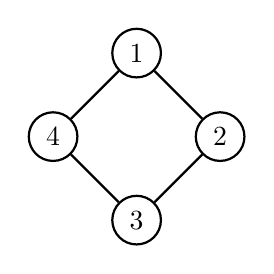
\begin{tikzpicture}[node distance={15mm}, thick, main/.style = {draw, circle}]
    \node[main] (1) {$1$};
    \node[main] (4) [below left of=1] {$4$};
    \node[main] (2) [below right of=1] {$2$};
    \node[main] (3) [below right of=4] {$3$};

    \draw (1) -- (2);
    \draw (2) -- (3);
    \draw (3) -- (4);
    \draw (4) -- (1);
\end{tikzpicture} 
        \caption{Graph $C_4$}
        \label{fig:c4}
    \end{figure}

    $1 = d_G(1,2) = d_G(2,3) = d_G(3,4) = d_G(4,1)$.

    $2 = d_G(1,3) = d_G(2,4)$.

    If $G = C_4$, then $d_G$ can be embedded in $\ell_1$ with no distortion.
    Embedding shown in figure~\ref{fig:c4_l1_embedding}.

    \begin{figure}[h]
        \centering
        \begin{tikzpicture}
    \begin{axis}[xmin=-1, xmax=1, ymin=-1, ymax=1, axis x line=middle, axis y line=middle]
        %\addplot[domain=-5:5]{2*x+2};
        %\addplot[domain=-5:5, color=red]{2*x+2};
        %\addplot[domain=-5:5, color=blue]{2*x+2};
        %\addplot[matk=*] coordinates {(2,2)};
        %\addplot[matk=*] coordinates {(0,0)};
        %\addplot[matk=*] coordinates {(-2,-2)};
        %\addplot[matk=*] coordinates {(0,2)};
        \node[label={180:{$X_1$}},circle,fill,inner sep=2pt] at (axis cs:-0.5,0.5) {};
        \node[label={180:{$X_2$}},circle,fill,inner sep=2pt] at (axis cs:0.5,0.5) {};
        \node[label={180:{$X_3$}},circle,fill,inner sep=2pt] at (axis cs:0.5,-0.5) {};
        \node[label={180:{$X_4$}},circle,fill,inner sep=2pt] at (axis cs:-0.5,-0.5) {};
    \end{axis}
\end{tikzpicture}
        \caption{$C_4$ embedding into $\ell_1$}
        \label{fig:c4_l1_embedding}
    \end{figure}

    Recall that
    \[ \cardinality{X-Y}_1 = \sum_{i=1}^{d} \cardinality{X_i - Y_i} \]

    Then,
    %\[ \cardinality{X_1 - X_2}_1 = \cardinality{X_2 - X_3}_1 = \cardinality{X_3 - X_4}_1 = \cardinality{X_1 - X_4}_1 = 1 \]
    %\[ \cardinality{X_1 - X_3}_1 = \cardinality{X_2 - X_4}_1 = 1+1 = 2 \]

    \begin{equation*}
        \begin{split}
            &\cardinality{X_1 - X_2}_1 = \cardinality{X_2 - X_3}_1 = \cardinality{X_3 - X_4}_1 = \cardinality{X_1 - X_4}_1 = 1\\
            &\cardinality{X_1 - X_3}_1 = \cardinality{X_2 - X_4}_1 = 1+1 = 2
        \end{split}
    \end{equation*}

    Thus, $f(i) = X_i$ is an embedding with no distortion.

    Say that now we want to embed $C_4$ into $\ell_2$.
    The embedding can be represented like the $\ell_1$ embedding (i.e. see figure~\ref{fig:c4_l1_embedding}).
    The difference with $\ell_1$, as it will be clear in a moment, is that points for which the shortest path is a diagonal, have a different distances in $\ell_2$ and $d_G$ (whereas in $\ell_1$ and $d_G$ it was the same).

    Recall that
    \[ \cardinality{X-Y}_2 = \sqrt{\sum_{i=1}^{d} (X_i - Y_i)^2} \]

    Then,
    %\[ \cardinality{X_1 - X_2}_2 = \cardinality{X_2 - X_3}_2 = \cardinality{X_3 - X_4}_2 = \cardinality{X_1 - X_4}_2 = 1 \]
    %\[ \cardinality{X_1 - X_3}_2 = \cardinality{X_2 - X_4}_2 = \sqrt{1^2 + 1^2} = \sqrt{2} \]

    \begin{equation*}
        \begin{split}
            &\cardinality{X_1 - X_2}_2 = \cardinality{X_2 - X_3}_2 = \cardinality{X_3 - X_4}_2 = \cardinality{X_1 - X_4}_2 = 1\\
            &\cardinality{X_1 - X_3}_2 = \cardinality{X_2 - X_4}_2 = \sqrt{1^2 + 1^2} = \sqrt{2}
        \end{split}
    \end{equation*}

    On the edges we have a distance of $1$. On the diagonals we have a distance of $\frac{2}{\sqrt{2}} = \sqrt{2}$.
    Thus, the distortion of this embedding is $\sqrt{2}$.

    Question: what is the minimum distortion of $C_4$ into $\ell_2$?

    \begin{theorem}
        The $C_4$-metric cannot be embedded into $\ell_2$ with distortion $< \sqrt{2}$.
    \end{theorem}

    \begin{proof}
        Let $f(i) = Y_i$ be an embedding for $i \in [4]$, and for $Y_i \in \mathbb{R}^d$.

        Let $M = \max (\cardinality{Y_1 - Y_2}_2, \cardinality{Y_2 - Y_3}_2, \cardinality{Y_3 - Y_4}_2, \cardinality{Y_1 - Y_4}_2)$ be the maximum edge length.

        Let $m = \min (\cardinality{Y_1 - Y_3}_2, \cardinality{Y_2 - Y_4}_2)$ be the minimum diagonal length.

        Lemma: $\forall Y_1, Y_2, Y_3, Y_4 \in \mathbb{R}^d$, $\cardinality{Y_1 - Y_3}_2^2 + \cardinality{Y_2 - Y_4}_2^2 \leq \cardinality{Y_1 - Y_2}_2^2 + \cardinality{Y_2 - Y_3}_2^2 + \cardinality{Y_3 - Y_4}_2^2 + \cardinality{Y_1 - Y_4}_2^2$.
        This is the "Short diagonals lemma", and its proof will be presented after the proof of this theorem.

        But then, the followings hold
        \[ 2m^2 \leq \cardinality{Y_1 - Y_3}_2^2 + \cardinality{Y_2 - Y_4}_2^2 \]
        \[ 4M^2 \geq \cardinality{Y_1 - Y2}_2^2 + \cardinality{Y_2 - Y_3}_2^2 + \cardinality{Y_3 - Y_4}_2^2 + \cardinality{Y_1 - Y_4}_2^2 \]

        Then,
        \[ 2m^2 \leq 4M^2 \rightarrow (\frac{m}{M})^2 \leq 2 \rightarrow \frac{m}{M} \leq \sqrt{2} \rightarrow m \leq M \sqrt{2} \]

        But we wanted $m = 2M$, thus the distortion has to be at least $\frac{2}{\sqrt{2}} = \sqrt{2}$.
    \end{proof}

    \begin{lemma}
        $\forall Y_1, Y_2, Y_3, Y_4 \in \mathbb{R}^d$,
        \[ \cardinality{Y_1 - Y_3}_2^2 + \cardinality{Y_2 - Y_4}_2^2 \leq \cardinality{Y_1 - Y_2}_2^2 + \cardinality{Y_2 - Y_3}_2^2 + \cardinality{Y_3 - Y_4}_2^2 + \cardinality{Y_1 - Y_4}_2^2 \]
    \end{lemma}

    \begin{proof}
        Recall that
        \[ \cardinality{Y_i - Y_j}_2^2 = \sum_{t} (Y_i(t) - Y_j(t))^2 \]

        We will prove our inequality on each coordinate independently.
        Consider a coordinate $t$, and let $z_i = Y_i(t) \in \mathbb{R}$.

        Claim: $(z_1 - z_2)^2 + (z_2 - z_3)^2 + (z_3 - z_4)^2 + (z_1 - z_4)^2 \geq (z_1 - z_3)^2 + (z_2 - z_4)^2$.

        Sum of Squares (SOS) Proof:
        $(z_1 - z_2)^2 + (z_2 - z_3)^2 + (z_3 - z_4)^2 + (z_4 - z_1)^2 - (z_1 - z_3)^2 - (z_2 - z_4)^2 = (z_1 - z_2 - z_3 - z_4)^2 \geq 0$
    \end{proof}


\subsection{Max-cover problem}

    Recall the problem~\nameref{subsect:setcover}.
    We now see a variation of it.

    Input: $C = \{ S \st S \subseteq [n] \} = \{ S_1, \dots, S_m \}$.

    Goal: find $C' \subseteq \binom{C}{k}$ s.t. $\cardinality{\bigcup_{S \in C'} S}$ is as large as possible.

    In algorithm \ref{alg:greedy_maxcover} a greedy algorithm for solving Max-cover.

    \begin{algorithm}
    \caption{Greedy for Max-cover}\label{alg:greedy_maxcover}
    \begin{algorithmic}%[1]
        \Procedure{Greedy}{$C,k$}
            \State~$C' \gets \emptyset$
            \State~$T_0 \gets \emptyset$

            \For{$i = 1,2, \dots, k$}
                \State~assign to each $S \in C \setminus C'$ the score $sc_{T_{i-1}}(S) = \cardinality{S \setminus T_{i-1}}$
                \State~let $S_i \in C \setminus C'$ be a set of largest $sc_{T_{i-1}}$ score
                \State~$C' \gets C' \cup \{ S_i \}$
                \State~$T_i \gets T_{i-1} \cup S_i$
            \EndFor
            
            \Return~$C'$
        \EndProcedure
    \end{algorithmic}
\end{algorithm}

    Recall that $1 - \frac{1}{e} \approx 0.63\dots$.

    \begin{theorem}
        \textsc{Greedy} returns a $(1 - \frac{1}{e})$-approximation to Max-cover.
    \end{theorem}

    \begin{proof}
        Let $C^* = \{ S_1^*, S_2^*, \dots, S_k^* \} \subseteq C$ be an optimal solution.

        Also, let $X^* = \bigcup_{i=1}^k S_i^*$ be the set of elements covered by $C^*$.
        Then $\textsc{OPT} = \cardinality{X^*}$.

        The algorithm picks sets $S_1, \dots, S_k$.
        Let $s_i$ be the score of $S_i$ when $S_i$ was picked (note that the score of a set $S_i$ can change during iterations, as more elements are covered).
        Then $s_i = \cardinality{S_i \setminus T_{i-1}}$, where $T_{i-1} = \bigcup_{j=1}^{i-1}S_j$.

        Also, let $t_i = \cardinality{T_i} = \bigcup_{j=1}^{i}S_j$.

        Let $u_i = \cardinality{X^*} - t_i$.

        Thus, we have defined the following values:
        \begin{itemize}
            \item $s_i$ is the number of "new" elements covered by $S_i$
            \item $t_i$ is the total number of elements covered by $S_1, \dots, S_i$
            \item $u_i$ is the advantage of the optimal solution over $S_1, \dots, S_i$
        \end{itemize}

        Then, $t_0 = 0$, and $t_k = \cardinality{T_k}$ is the value of $C'$ (the solution returned by the greedy procedure).
        Also $u_0 = \cardinality{X^*} - t_0 = \textsc{OPT}$.

        We want to prove that $t_k \geq (1 - \frac{1}{e})u_0$.

        Claim: $s_i \geq \frac{u_{i-1}}{k}$, $\forall i \in \{ 1, \dots, k \}$.

        Proof of the claim.
        The set $S = S_i$ chosen by greedy maximizes $\cardinality{S \setminus T_{i-1}}$.
        At least one set $S_j^* \in C^*$ must cover at least $\frac{u_{i-1}}{k} = \frac{\cardinality{X^*} - \cardinality{T_{i-1}}}{k}$ elements of $X^* \setminus T_{i-1}$.

        If it was not the case, it would be impossible for $C^*$ to cover all of $X^* \setminus T_{i-1}$.
        In fact, the set has cardinality $u_{i-1}$, and $\cardinality{C^*} = k$. Also $C^*$ has to cover all of $X^* \setminus T_{i-1}$, since the latter is a subset of $X^*$.

        Then, $\exists S_j^* \in C^*$ s.t. $sc_{T_{i-1}}(S_j^*) = \cardinality{S_j^* \setminus T_{i-1}} \geq \frac{u_{i-1}}{k}$.
        Then, $sc_{T_{i-1}}(S_i) \overset{\text{(greedy choice)}}{\geq} sc_{T_{i-1}}(S_j^*) \geq \frac{u_{i-1}}{k}$, and $s_i = sc_{T_{i-1}}(S_i)$. And this proves the claim.

        Claim: $u_i \leq (1 - \frac{1}{k})^i \cardinality{X^*}$, for $i \in \{ 0, \dots, k \}$.

        By induction on $i$.

        Base case ($i=0$). $u_0 = \cardinality{X^*}$.

        Inductive case. Assume the claim holds until $i \leq k-1$; we want to prove it for $i+1$.

        %$u_{i+1} = \cardinality{X^*} - t_{i+1} = \cardinality{X^*} - \cardinality{T_{i+1}} = \cardinality{X^*} - \cardinality{\bigcup_{j=1}^{i+1} S_j} =
        %\cardinality{X^*} - \cardinality{\bigcup_{j=1}^{i} S_j} - \cardinality{S_{i+1} \setminus \bigcup_{i=1}^i S_j} = \cardinality{X^*} - \cardinality{T_i} - \cardinality{S_{i+1} \setminus T_i} =
        %\cardinality{X^*} - \cardinality{T_i} - s_{i+1} = u_i - s_{i+1} \overset{\text{previous claim}}{\leq} u_i - \frac{u_i}{k} = (1 - \frac{1}{k})u_i \leq
        %(1 - \frac{1}{k}) - (1 - \frac{1}{k})^i \cardinality{X^*} = (1 - \frac{1}{k})^{i+1} \cardinality{X^*}$.
        
        \begin{equation*}
            \begin{split}
                u_{i+1} &= \cardinality{X^*} - t_{i+1} = \cardinality{X^*} - \cardinality{T_{i+1}} = \cardinality{X^*} - \cardinality{\bigcup_{j=1}^{i+1} S_j} =\\
                        &= \cardinality{X^*} - \cardinality{\bigcup_{j=1}^{i} S_j} - \cardinality{S_{i+1} \setminus \bigcup_{i=1}^i S_j} = \cardinality{X^*} - \cardinality{T_i} - \cardinality{S_{i+1} \setminus T_i} =\\
                        &= \cardinality{X^*} - \cardinality{T_i} - s_{i+1} = u_i - s_{i+1} \overset{\text{previous claim}}{\leq} u_i - \frac{u_i}{k} = (1 - \frac{1}{k})u_i \leq\\
                        &\leq (1 - \frac{1}{k}) - (1 - \frac{1}{k})^i \cardinality{X^*} = (1 - \frac{1}{k})^{i+1} \cardinality{X^*}
            \end{split}
        \end{equation*}

        And this proves the claim.

        Then, $u_k \leq (1 - \frac{1}{k})^k \cardinality{X^*} \leq (1 - \frac{1}{e}) \cardinality{X^*} \leq \frac{1}{e} \cardinality{X^*}$.
        But, $u_k = \cardinality{X^*} - \cardinality{T_k}$, then $\cardinality{X^*} - \cardinality{T_k} = u_k \leq \frac{1}{e} \cardinality{X^*}$, then $(1 - \frac{1}{e}) \cardinality{X^*} \leq \cardinality{T_k} = t_k$.
        
    \end{proof}


\subsection{Set functions}
    Given $S \subseteq [n]$, a set function is a function $f : 2^{[n]} \rightarrow \mathbb{R}$, where $f(S)$ is the value of $f$ at $S$.

    Set functions can be divided in three kinds.

    \textbf{Submodular functions}, $\forall S,T \subseteq [n]$:
    \[ f(S) + f(T) \geq f(S \cup T) + f(S \cap T) \]

    \textbf{Modular functions}, $\forall S,T \subseteq [n]$:
    \[ f(S) + f(T) = f(S \cup T) + f(S \cap T) \]
    Also, a function is modular iff $\exists$ weights $w_1, \dots, w_n, z$ s.t. $f(S) = z + \sum_{i \in S} w_i$.

    \textbf{Supermodular functions}, $\forall S,T \subseteq [n]$:
    \[ f(S) + f(T) \leq f(S \cup T) + f(S \cap T) \]

    Let us consider the following set function.
    Let $C = \{ A_1, \dots, A_n \}$, where $A_i \subseteq [t]$.
    Let our "covering" function be
    \[ f(S) = \cardinality{\bigcup_{j \in S} A_j} \]
    for $S \subseteq [n]$.

    \begin{theorem}
        The function $f$, as just defined, is submodular.
    \end{theorem}

    \begin{proof}
        Observe that $f(S) = \sum_{i \in [t]} [\exists j \in S : i \in A_j] = \sum_{i=1}^{t} f_i(S)$, where
        \begin{equation}
            f_i(S) =
            \begin{cases}
                1 & \text{if } \exists j \in S \text{ s.t. } i \in A_j\\
                0 & \text{o/w}
            \end{cases}
        \end{equation}

        We claim that, $\forall i \in [t]$, $f_i$ is submodular.
        To prove it, we need to prove that $f_i(S) + f_i(T) \geq f_i(S \cup T) + f_i(S \cap T)$, $\forall S,T \subseteq [n]$.

        Since the range of $f_i$ is (a subset of) $\B$, if $f_i(S \cup T) = f_i(S \cap T) = 0$, then the inequality holds trivially.

        Moreover, $f_i$ is monotone increasing: if $S \subseteq T$, then $f(S) \leq f(T)$.
        If $f_i(S) = 1$, then $\exists j \in S$ s.t. $i \in A_j$. Since $j \in S \subseteq T$, then it must be that $f_i(T) = 1$.

        Thus we only need to consider two cases:
        \begin{itemize}
            \item[a.] $f_i(S \cup T) = f_i(S \cap T) = 1$
            \item[b.] $f_i(S \cap T) = 0$ and $f_i(S \cup T) = 1$
        \end{itemize}

        If a. holds, then $\exists j \in S \cap T$ s.t. $i \in A_j$, but then $j \in S$ and $j \in T$, thus $f_i(S) = f_i(T) = 1$

        if b. holds, then $\exists j \in S \cup T$ s.t. $i \in A_j$, thus $f_i(S \cup T) = 1$. Either $j \in S$ or $j \in T$, and not both. Thus $f_i(S) + f_i(T) = 1$.

        Thus, we have proved that $\forall i \in [t]$, $f_i$ is submodular.
        To finish the proof we have to show that the sum of submodular functions is submodular.

        $f(S) = \sum_{i=1}^{t} f_i(S)$·

        Let $S,T \subseteq [n]$, then $f(S) + f(T) = \sum_{i=1}^{t} (f_i(S) + f_i(T)) \overset{f_i \text{ submodular}}{\geq} \sum_{i=1}^{t}(f_i(S \cup T) + f_i(S \cap T)) = \sum_{i=1}^{t} f_i(S \cup T) + \sum_{i=1}^{t} f_i (S \cap T) = f(S \cup T) + f(S \cap T)$.
    \end{proof}

    We now study Max-cover as being a special case of submodular functions.

    Submodular functions are also studied in economics, where they are given a different name.
    \begin{definition}[Diminishing return]
        Given $S \subseteq [n]$ and $x \in [n] \setminus S$, we define the return of $x$ at $S$ to be
        \[ \Delta_f (x \st S) = f(S \cup \{ x \}) - f(S) \]
        That is, how much do I gain by adding $x$ to $S$.
    \end{definition}

    A function $f$ has the diminishing return property if, $\forall S \subseteq T$, $\forall x \in [n] \setminus T$:
    \[ \Delta_f(x \given S) \geq \Delta_f(x \given T) \]

    \begin{lemma}
        If $f$ is submodular then $f$ has the diminishing return property.
    \end{lemma}

    \begin{proof}
        We'd like to prove that $\forall A \subseteq B$, $\forall x \in [n] \setminus B$, $\Delta_f(x \given A) \geq \Delta_f(x \given B)$.

        Let us define $S = A \cup \{x\}$, $T = B$.

        By submodularity of $f$, $f(S) + f(T) \geq f(S \cup T) + f(S \cap T)$.
        Thus $f(A \cup \{x\}) + f(B) \geq f(A \cup \{x\} \cup B) + f((A \cup \{x\}) \cap B)$.

        $f(A \cup \{x\}) + f(B) \geq f(B \cup \{x\}) + f(A)$

        $f(A \cup \{x\}) - f(A) \geq f(B \cup \{x\}) - f(B)$

        Then, $\Delta_f(x \given A) \geq \Delta_f(x \given B)$.
    \end{proof}

    \begin{exercise}
        The converse of previous lemma also holds.
        Prove that if $f$ has the diminishing return property, then $f$ is submodular.
    \end{exercise}

    We aim to maximize a submodular $f$ under a "cardinality constraint".
    In Max-cover, we wanted to maximize $f(S)$ under $\cardinality{S} = k$.

    In algorithm~\ref{alg:greedy_submodular}

    \begin{algorithm}
    \caption{Submodular functions framework for Max-cover}\label{alg:greedy_submodular}
    \begin{algorithmic}%[1]
        \Procedure{$\textsc{Greedy}_f$}{$X,k$}
            \State~$S_0 \gets \emptyset$

            \For{$i = 0,1, \dots, k-1$}
                \State~let $x_{i+1} \in X$ be a maximizer of $f(S_i \cup \{x_{i+1}\})$  %\Comment{equiv. to max of $\Delta_f(x_{i+1} \given S_i)}
                \State~$S_{i+1} \gets S_i \cup \{x_{i+1}\}$
            \EndFor
            
            \Return~$S_k$
        \EndProcedure
    \end{algorithmic}
\end{algorithm}

    \begin{theorem}
        If $f$ is submodular, monotone and non-negative, then $\textsc{Greedy}_f(X,k)$ returns a $(1 - \frac{1}{e})$-approximation to $\max_{S \in \binom{X}{k}} f(S)$.
    \end{theorem}

    \begin{proof}
        Let $S^* = \{ X_1^*, \dots, X_k^* \}$ be an optimal solution.
        
        Then $f(S^*) = \max_{S \in \binom{X}{k}} f(S)$.

        $\forall i = 0, \dots, k-1$:
        %\begin{multline*}
        %    f(S^*) \overset{\text{monotonicity}}{\leq} f(S^* \cup S_i) =\\
        %    f(\{ X_1^*, \dots, X_k^* \} \cup S_i) - f(\{ X_1^*, \dots, X_{k-1}^*\} \cup S_i) + f(\{ X_1^*, \dots, X_{k-1}^* \} \cup S_i) -\\
        %    f(\{ X_1^*, \dots, X_{k-2}^* \} \cup S_i)  + f(\{ X_1^*, \dots, X_{k-2}^* \} \cup S_i)  - \cdots - f(\{ X_1^*, X_2^*\} \cup S_i) + \\
        %    f(\{ X_1^*, X_2^*\} \cup S_i)  - f({X_1^*} \cup S_i) + f({X_1^*} \cup S_i) - f(S_i) + f(S_i) =\\
        %    \Delta_f(X_{k}^* \given S_i \cup \{ X_1^*, \dots, X_{k-1}^* \}) +\\
        %    \Delta_f(X_{k-1}^* \given S_i \cup \{ X_1^*, \dots, X_{k-2}^* \}) +\\
        %    \vdots\\
        %    \Delta_f(X_{2}^* \given S_i \cup \{ X_1^*\}) +\\
        %    \Delta_f(X_{1}^* \given S_i) +\\
        %    f(S_i) =\\
        %    f(S_i) + \sum_{j=1}^{k} \Delta_f(X_j^* \given S_i \cup \{ X_1^*, \dots, X_{j-1}^* \}) \overset{\text{diminish. return}}{\leq} f(S_i) + \sum_{j=1}^{k} \Delta_f(X_j^* \given S_i) \overset{\text{greedy choice}}{\leq}\\
        %    f(S_i) + \sum_{j=1}^{k} \Delta_f(X_{i+1} \given S_i) = f(S_i) + k \cdot \Delta_f(X_{i+1} \given S_i) = f(S_i) + k (f(S_i \cup \{ X_{i+1} \}) - f(S_i))
        %\end{multline*}

        \begin{equation*}
            \begin{split}
                f(S^*) \overset{\text{monotonicity}}{\leq} & f(S^* \cup S_i) =\\
                    &= f(\{ X_1^*, \dots, X_k^* \} \cup S_i) - f(\{ X_1^*, \dots, X_{k-1}^*\} \cup S_i) + f(\{ X_1^*, \dots, X_{k-1}^* \} \cup S_i) -\\
                    &- f(\{ X_1^*, \dots, X_{k-2}^* \} \cup S_i)  + f(\{ X_1^*, \dots, X_{k-2}^* \} \cup S_i)  - \cdots - f(\{ X_1^*, X_2^*\} \cup S_i) + \\
                    &+ f(\{ X_1^*, X_2^*\} \cup S_i)  - f({X_1^*} \cup S_i) + f({X_1^*} \cup S_i) - f(S_i) + f(S_i) =\\
                    &= \Delta_f(X_{k}^* \given S_i \cup \{ X_1^*, \dots, X_{k-1}^* \}) +\\
                    &+ \Delta_f(X_{k-1}^* \given S_i \cup \{ X_1^*, \dots, X_{k-2}^* \}) +\\
                    & \vdots\\
                    &+ \Delta_f(X_{2}^* \given S_i \cup \{ X_1^*\}) +\\
                    &+ \Delta_f(X_{1}^* \given S_i) +\\
                    &+ f(S_i) =\\
                    &= f(S_i) + \sum_{j=1}^{k} \Delta_f(X_j^* \given S_i \cup \{ X_1^*, \dots, X_{j-1}^* \}) \overset{\text{diminish. return}}{\leq}\\
                    &\leq f(S_i) + \sum_{j=1}^{k} \Delta_f(X_j^* \given S_i) \overset{\text{greedy choice}}{\leq}\\
                    &\leq f(S_i) + \sum_{j=1}^{k} \Delta_f(X_{i+1} \given S_i) = f(S_i) + k \cdot \Delta_f(X_{i+1} \given S_i) =\\
                    &= f(S_i) + k (f(S_i \cup \{ X_{i+1} \}) - f(S_i))
            \end{split}
        \end{equation*}

        Then, $f(S^*) \leq f(S_i) + k (f(S_i \cup \{ X_{i+1} \}) - f(S_i))$.

        Let us define $\delta_i = f(S^*) - f(S_i)$.

        $f(S^* - f(S_i)) \leq k (f(S_{i+1}) - f(S_i))$

        $\delta_i \leq k (-f(S^*) + f(S_{i+1}) - f(S_i) + f(S^*))$

        $\delta_i \leq k (\delta_i - \delta_{i+1})$

        $k \delta_{i+1} \leq (k-1) \delta$

        Then, $\forall i = 0, \dots, k-1$, $\delta_{i+1} \leq (1 - \frac{1}{k}) \delta_i$.

        Finally,
        %$\delta_0 = f(S^*) - f(S_0) = f(S^*) - f(\emptyset) \overset{\text{non-neg.}}{\leq} f(S^*)$
        %$\delta_1 \leq (1 - \frac{1}{k}) \delta_0 \leq (1 - \frac{1}{k}) f(S^*)$
        %$\delta_2 \leq (1 - \frac{1}{k}) \delta_1 \leq (1 - \frac{1}{k})^2 f(S^*)$
        %$\vdots$
        %$\delta_k \leq f(S^*) - f(S_k) \leq (1 - \frac{1}{k})^k f(S^*) \leq \frac{1}{e} f(S^*) \rightarrow f(S_k) \geq (1 - \frac{1}{e}) f(S^*)$

        \begin{equation*}
            \begin{split}
                &\delta_0 = f(S^*) - f(S_0) = f(S^*) - f(\emptyset) \overset{\text{non-neg.}}{\leq} f(S^*)\\
                & \delta_1 \leq (1 - \frac{1}{k}) \delta_0 \leq (1 - \frac{1}{k}) f(S^*)\\
                & \delta_2 \leq (1 - \frac{1}{k}) \delta_1 \leq (1 - \frac{1}{k})^2 f(S^*)\\
                & \vdots\\
                & \delta_k \leq f(S^*) - f(S_k) \leq (1 - \frac{1}{k})^k f(S^*) \leq \frac{1}{e} f(S^*) 
            \end{split}
        \end{equation*}

        Then, $f(S_k) \geq (1 - \frac{1}{e}) f(S^*)$.
    \end{proof}